% !TEX TS-program = pdflatex
% !TEX encoding = UTF-8 Unicode

\documentclass{beamer}


\mode<presentation>
{
  \usetheme{Warsaw}
  \setbeamercovered{transparent}
  \useoutertheme{infolines}
  \setbeamertemplate{headline}[infolines theme]
  \setbeamertemplate{caption}[numbered]
  \setbeamertemplate{footline}[split theme,frame number]
  \setbeamerfont{footnote}{size=\scriptsize}
}

\usepackage[english]{babel} % or whatever
\usepackage[utf8]{inputenc} % or whatever
\usepackage{times}
\usepackage[T1]{fontenc}
% Or whatever. Note that the encoding and the font should match. If T1
% does not look nice, try deleting the line with the fontenc.

% Added packages
\usepackage{natbib}
\usepackage{cleveref}
\usepackage{url}
\usepackage{tikz-cd}
\tikzcdset{scale cd/.style={every label/.append style={scale=#1},
    cells={nodes={scale=#1}}}}
\usepackage[center]{caption}
\usepackage{subcaption}

% Two-Column Layouts
\def\begincols{\begin{columns}}
\def\begincol{\begin{column}}
\def\endcol{\end{column}}
\def\endcols{\end{columns}}

%\let\cite\citep
\renewcommand{\cite}{\citep}
% from \citep to \cite to cite in author style, e.g. [Mule, 2008]

% \bibliographystyle{plainnat}
%\citep: citation in parentheses, e.g. [Mule, 2008]
%\citet: citation as author, e.g. Mule [2008]
%\cite: citation as author, \citet by default 

\title [Text Preprocessing Methods] % (optional, use only with long paper titles)
{Guidelines in Selecting Appropriate\\ Text Preprocessing Methods}

\author [chrchai@microsoft.com] %[Christine P. Chai] %[Author, Another] % (optional, use only with lots of authors)
{Christine P. Chai}
% {F.~Author\inst{1} \and S.~Another\inst{2}}
% - Give the names in the same order as the appear in the paper.
% - Use the \inst{?} command only if the authors have different
%   affiliation.

\institute[]
{Microsoft\\ chrchai@microsoft.com}

%\institute[Duke Stat] % (optional, but mostly needed)
%{
  %\inst{1}%
  %Department of Statistical Science\\
  %Duke University
  %\and
  %\inst{2}%
  % - Use the \inst command only if there are several affiliations.
% - Keep it simple, no one is interested in your street address.
%}

\date[tinyurl.com/csp-2021-chai] % (optional, should be abbreviation of conference name)
{Conference on Statistical Practice (CSP) 2021\\ \vspace{40pt}
\footnotesize{Slides on GitHub: \url{https://tinyurl.com/csp-2021-chai}}}
% - Either use conference name or its abbreviation.
% - Not really informative to the audience, more for people (including
%   yourself) who are reading the slides online

\newenvironment{changemargin}[2]{%
  \begin{list}{}{%
    \setlength{\topsep}{0pt}%
    \setlength{\leftmargin}{#1}%
    \setlength{\rightmargin}{#2}%
    \setlength{\listparindent}{\parindent}%
    \setlength{\itemindent}{\parindent}%
    \setlength{\parsep}{\parskip}%
  }%
  \item[]}{\end{list}} 

\begin{document}

\begin{frame}
  \titlepage
\end{frame}

% This presentation is 10-15 minutes.

% Suppress the outline slide AFTER I have completed the whole slide deck.
%\begin{frame}{Outline}
  %\tableofcontents[hidesubsections]
  % You might wish to add the option [pausesections]
%\end{frame}

% The first draft does not have to be perfect; it just has to be complete!

\section{Introduction}

\begin{frame}{Why is \textbf{\color{yellow}data} preprocessing important?}
\begin{itemize}
\item Data scientists spend more than 50\% of their work time on data preprocessing, i.e., preparing the data for analysis.\\
\begin{flushright}
-- \textit{The New York Times}~\cite{lohr2014bigdata}
\end{flushright}
	\bigskip
\item Although time-consuming, data preprocessing is worth the efforts. Real-life data are messier than people think!~\cite{chai2020importance}\\
	Adequately preprocessed data are key to success in modeling.
% e.g. Outliers may come from data entry mistakes.
% Data errors are inevitable and may occur in creative and unexpected ways.
	\bigskip
\item Data can be structured (numeric) and/or unstructured (text).
\item There is no one-size-fits-all solution for data preprocessing!
\end{itemize}
\end{frame}

\begin{frame}{Why is \textbf{\color{yellow}text} preprocessing important?}
\begin{itemize}
\item ``Merrill Lynch recently estimated that more than 80\% of all potentially useful business information is unstructured data.''~\cite{gharehchopogh2011analysis}
	\bigskip
\item Text data also require appropriate preprocessing,\\ to prepare the corpus for machine learning and text mining models.~\cite{kalra2018importance}
	\bigskip
\item Webscraped text often contains lots of HTML formats.\\
	$\Rightarrow$ Remove using Python \texttt{BeautifulSoup} or $\mathsf{R}$ \texttt{textclean}.
\item Application-specific formats: e.g. [10:23 PM] in chat messages\\
	$\Rightarrow$ Remove these formats using regular expressions.
\end{itemize}
\end{frame}

\begin{frame}{Text preprocessing is more important than it seems!}
\begin{itemize}
% Reproducibility + documentation
\item Text preprocessing details affect \textbf{reproducibility}.{\small~\cite{roy2018clean}}
\item Removing stopwords: Which words are regarded as stopwords?\\
	Obvious words: ``I'', ``the'', etc. What about non-obvious words?\\
	e.g. Is ``algorithm'' a stopword in a computer science corpus?
	\bigskip
\item\citet{trieschnigg2007influence}: \textbf{Tokenization decisions} can contribute more to system performance than the text model itself.
% Original sentence: ``Tokenization decisions can contribute more to system performance than the algorithm itself.'' The algorithm means the machine learning model.
	\bigskip
\item Text string \texttt{NF-$\kappa$ B/CD28-responsive} can be tokenized in many ways, resulting in different precision for document retrieval:
	\begin{itemize}
	\small
	\item \texttt{nf $\kappa$ b cd responsive}: 32\% precision
	\item \texttt{NF-$\kappa$ B/CD28-responsive} (non-whitespace): 17\%
	\item \texttt{nf kappa nfkappa b cd 28 respons bcd28respons}: 40\%
	\end{itemize}
\end{itemize}
\end{frame}

% ~\citet{trieschnigg2007influence} also pointed out that tokenization decisions can contribute more to system performance than the algorithm itself. The text string ``NF-$\kappa$ B/CD28-responsive'' has at least 12 different kinds of tokenization results, depending on the preprocessing techniques used. The various approaches in tokenization resulted in up to 46\% difference in the precision for document retrieval.

\begin{frame}{Tokenization Choices Matter: Another Example}
\begin{itemize}
\item Tokenization choices of the gene name \textit{alpha-2-macroglobulin} lead to different results of pattern matching in biomedical text.
\end{itemize}
\begin{figure}[!ht]
	\centering
	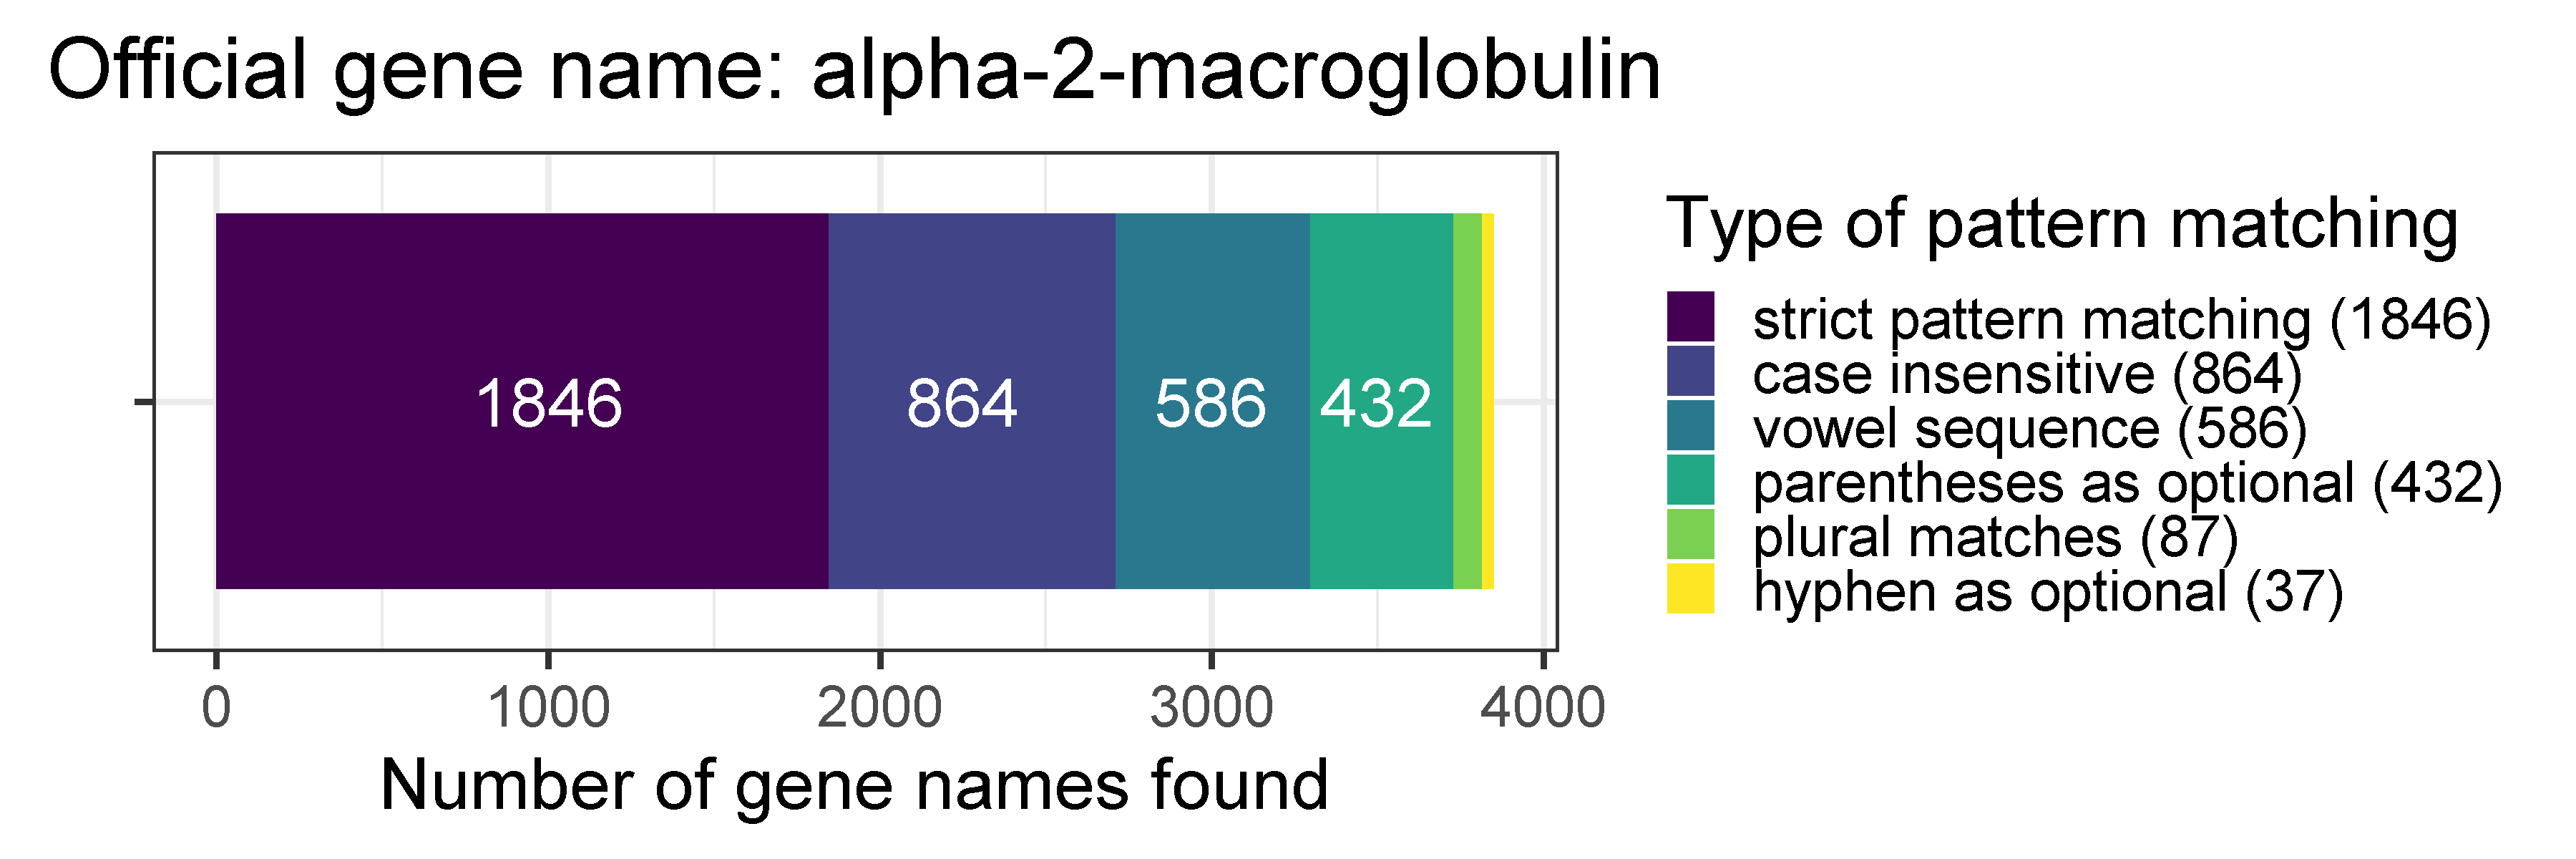
\includegraphics[width=\textwidth]{Figures/cohen2002_table2_legend.png}
	%\caption{write the title here}
\end{figure}
\begin{flushright}
Data from Table 2 in~\cite{cohen2002contrast}
\end{flushright}
\end{frame}

\begin{frame}{Text Preprocessing: Resources $\neq$ Guidelines}
\begin{itemize}
\item Lots of resources:
	\begin{itemize}
	\item NLTK in Python (Natural Language Toolkit)~\cite{bird2009natural}
	\item $\mathsf{R}$ packages: \texttt{stringr}, \texttt{quanteda}, \texttt{textclean}, \texttt{tm}, etc.
	\item SAS Text Miner, Microsoft Azure Machine Learning Studio
	\end{itemize}
\item But most are for implementation (\textbf{how}), not for guidelines (\textbf{why}).
	\bigskip
\item Unanswered questions include and are not limited to:
	\begin{itemize}
	\item Which methods are better for which text applications? % NLP
	\item How to improve the current text preprocessing pipeline?
	\item What are the potential risks of a specific method?
	\end{itemize}
\end{itemize}
\end{frame}

\begin{frame}{Structure of this talk: Text Preprocessing Methods}
\begin{itemize}
\item Discuss several commonly-used methods\\
	Explain the advantages and potential issues
\item Review specific examples of text analysis\\
	How preprocessing decisions contribute to the modeling
\item Discussion and key takeaways % on text preprocessing
	\bigskip
\item But before we get into the methods, let's talk about the\\ 
	recent advances in natural language processing.
\end{itemize}
\end{frame}

\begin{frame}{Recent Advances in Natural Language Processing}
\begin{itemize}
\item Lots of pretrained word embeddings for text models:\\
\texttt{word2vec}~\cite{mikolov2013efficient}, \texttt{GloVe}~\cite{pennington2014glove}, \\
\texttt{BERT}~\cite{devlin2018bert}, \texttt{ELMo}~\cite{peters2018deep}, etc.
\item Word embeddings map words to vectors using a large corpus.
\item Helpful for text models and support in multiple languages.
	\bigskip
\item We still need to learn text preprocessing methods, because \textbf{word embeddings are not a panacea}, i.e., have some limitations.
	\begin{itemize}
	\item Tokenization is required to break a text string into tokens (words).
	% Without tokenization, we don't have words in the first place!
	\item Some minority languages (e.g. Tibetan) are not supported yet.\footnote{\url{https://github.com/google-research/bert/blob/master/multilingual.md}}
	\item To add extra words (e.g. company-specific acronyms),\\ 
	we may need to retrain the word embeddings.~\cite{wilson2020urban}
	\end{itemize}
\end{itemize}
\end{frame}

\section{Common Text Preprocessing Methods}

%\frame{\tableofcontents[currentsection]}
\frame{\tableofcontents[currentsection, hidesubsections]}

\subsection{Tokenization}

\begin{frame}{Tokenization: Implementation}
\begin{itemize}
\item Convert a text string into a sequence of words (tokens)
\item Whitespace is not the only separator.~\cite{clough2001perl}
\item Tools: Python \texttt{nltk.tokenize}, $\mathsf{R}$ \texttt{str$\_$split} in \texttt{stringr} 
	\bigskip
\item Example 1: ``Statistics is fun'' $\Rightarrow$ ``Statistics'', ``is'', ``fun''
\item Example 2: ``I downloaded this software on-the-fly''\\
	Does ``on-the-fly'' count as one word or three words?
	\bigskip
\item We need to \textbf{decide which characters count as separators}.
\item Examine abbreviations and non-standard punctuation usage, especially in biomedical text.~\cite{diaz2015analysis}
\item And most importantly, be clear and consistent with the definitions.
\end{itemize}
\end{frame}

\begin{frame}{Tokenization: Need Precise Definitions}
\begin{itemize}
\item \textbf{Lexical richness} measures the quality of vocabulary in a corpus~\cite{malvern2012measures}. It can be defined by
$$\textbf{type-token ratio} =  \dfrac{\text{the number of types (distinct words)}}{\text{the number of tokens (total words)}}$$
\item But the terms ``type'' and ``token'' are loosely defined.\\
e.g. ``don't'' vs ``do not'', ``New$\_$York'' vs ``New York''
	\bigskip
% Keep this sentence because I really want to emphasize the problem of p-hacking.
\item Some researchers try various definitions and select one that produces a statistically significant result.~\cite{cohen2019p-hacking}
\item\textbf{P-hacking hurts reproducibility in research!}~\cite{head2015extent}
\item Good practice: Give the precise definition of ``type'' and ``token''
\end{itemize}
\end{frame}

% Main paper:~\cite{barrett2011building}
\begin{frame}{Tokenization: Compound Words}
\begin{itemize}
\item Compound words in languages with whitespace between tokens
	\begin{itemize}
	\item ``White House'' in English, ``sin embargo'' (however) in Spanish, ``parce que'' (because) in French~\cite{barrett2011building}
	\item In Arabic, a word has up to four independent tokens.~\cite{attia2007arabic}
	\end{itemize}
	\bigskip
\item Traditional approach: Find the terms that are statistically and practically significant~\cite{blei2009visualizing}
\item Modern approach: Leverage contextualized word representations to find the compound words~\cite{shwartz2019still}
	\bigskip
% Languages that contain whitespace between words
% Consider: N-gramming and multi-word expressions
% // but don't remove that section!
\item CJK (Chinese, Japanese, Korean) do not have whitespaces, and a word can also contain multiple tokens.
\item Possible to train a neural network model on known words, and update the model based on new information.~\cite{hiraoka2019stochastic}
%\item For Korean text, researchers have also decomposed characters into basic Korean alphabet for compression~\cite{moon2020jamo}.
\end{itemize}
\end{frame}


\subsection{Handling Punctuation}
% Easiest way: Remove all punctuation
% But not the only way :)

\begin{frame}{Handling Punctuation}
\begin{itemize}
\item Easiest way is to remove all punctuation from the text corpus.
	\begin{itemize}
	\item Acceptable for information retrieval \& topic modeling, where we focus on text rather than sentence~\cite{korde2012text}.
	\item Inappropriate for applications that require sentence segmentation!
	\end{itemize}
	\bigskip
\item \textbf{Punctuation provides syntactic information for parsing.}
\item Categories: sentence-final, sentence-internal, word-internal
\item Part-of-speech tagging needs to identify sentence boundaries first.
\item Sentences are necessary for end-use applications, such as:\\
\textbf{text summarization, machine translation, question answering}.\\
~\cite{patil2015automatic, kim2019researching, li2001incorporating}
\end{itemize}
\end{frame}

% ---------------------------------------------------------------------------

% When we separate a string into shorter strings via punctuation, discourse parsing is also of interest to understand the hierarchical and syntactic structure of the text string~\cite{soricut2003sentence, peldszus2015joint}.

\begin{frame}[fragile]{Punctuation Serves as Discourse Markers}
Discourse parsing needs punctuation to identify relations between text.
\vspace{-20pt}
\begin{flushright}
~\cite{ji2014representation}
\end{flushright}

\begincols
  \begincol{.50\textwidth}
\begin{itemize}
\item ``A panda eats shoots and leaves.'' (without comma)
\end{itemize}
  \endcol
  \begincol{.50\textwidth}
\begin{itemize}
\item ``A panda eats\textbf{,} shoots and leaves.'' (with comma)
\end{itemize}
  \endcol
\endcols

\vspace{-30pt}
% https://tikzcd.yichuanshen.de/
% Figure caption: Hierarchical structure of a sentence with or without a comma.

\begincols
  \begincol{.50\textwidth}
\begin{figure}[!ht]
\[
\begin{tikzcd}[scale cd=0.80]
                                          & \framebox[1.1\width]{A panda} \arrow[d]          &        \\
                                          & \framebox[1.1\width]{eats} \arrow[ld] \arrow[rd] &        \\
\framebox[1.1\width]{shoots} \arrow[rr, "\text{and}", no head, dotted] &         & \framebox[1.1\width]{leaves}
\end{tikzcd}
\]
\end{figure}
  \endcol
  \begincol{.50\textwidth}
\begin{figure}[!ht]
\[
\begin{tikzcd}[scale cd=0.80]
                                       & \framebox[1.1\width]{A panda} \arrow[ld] \arrow[d] \arrow[rd]  &        \\
\framebox[1.1\width]{eats} \arrow[r, "{\textbf{,}}", no head, dotted] & \framebox[1.1\width]{shoots} \arrow[r, "\text{and}", no head, dotted] & \framebox[1.1\width]{leaves}  
\end{tikzcd}
\]
\end{figure}
  \endcol
\endcols

\begin{flushright}
\footnotesize
-- \textit{Eats, Shoots \& Leaves: The zero tolerance approach to punctuation} by~\citet{truss2004eats}
\end{flushright}

\end{frame}

% ---------------------------------------------------------------------------

\begin{frame}[fragile]{Removing Punctuation}
\begin{itemize}
\item If we decide to remove punctuation from the corpus,\\ 
	using regular expressions is straightforward.
\item Python and $\mathsf{R}$ both provide the list of punctuation symbols:\\ 
	\begin{verbatim} 
	!"#$\%&'()*+,-./:;<=>?@[\]^_`{|}~ 
	\end{verbatim}
	\bigskip
\item Beware of word-internal punctuation for contractions
\item Predefined list to split contractions\footnote{\url{https://gist.github.com/nealrs/96342d8231b75cf4bb82}} (e.g. ``don't'' $\Rightarrow$ ``do not'')
\item Python \texttt{pycontractions} provides higher precision with context\\
	e.g. Does ``I'd'' map to ``I would'' or ``I had''?~\cite{pycontractions}
	\bigskip
\item Consider retaining emoticons (:-), :p) with Python NLTK's \texttt{TweetTokenizer()}, especially in social media data
% \item Repeated punctuation (!!, ??) shows stronger emotions => sentiment analysis
\end{itemize}
\end{frame}

\subsection{Removing Stopwords}

\begin{frame}{Removing Stopwords: Overview}
\begin{itemize}
\item Stopwords are the words that \textbf{do not distinguish one document from another in the corpus}.~\cite{ferilli2014automatic}
	\begin{itemize}
	\item General: prepositions (``at''), pronouns (``you''), articles (``the''), etc.
	\item Domain-specific: ``method'', ``problem'', ``algorithm'' in a corpus of machine learning papers~\cite{fan2017promoting}
	\end{itemize}
	\bigskip
\item\textbf{Don't just regard stopwords as ``noise''.}\\ 
	Every word has semantic meaning, no matter how little.
	\bigskip
\item Stopwords are identified from a predefined list, or from corpus:
	\begin{itemize}
	\item TF-IDF (term frequency -- inverse document frequency) 
	% balances the frequency and the distinguishability of words in a corpus.
	\item Entropy (information theory)~\cite{gerlach2019universal}
	\item Kullback-Leibler (KL) divergence~\cite{sarica2020stopwords}
	\end{itemize}
\item Especially useful for text corpora with technical content
\end{itemize}
\end{frame}

\begin{frame}{English Classic Novel: \textit{Wuthering Heights}}
% Information Retrieval: Remove stopwords first
\begin{itemize}
\item Most frequent words are stopwords: and, the, I, etc.
\item Zipf's law: The frequency distribution is right-skewed.~\cite{zipf1949human}
\end{itemize}
\begin{figure}[!ht]
	\centering
	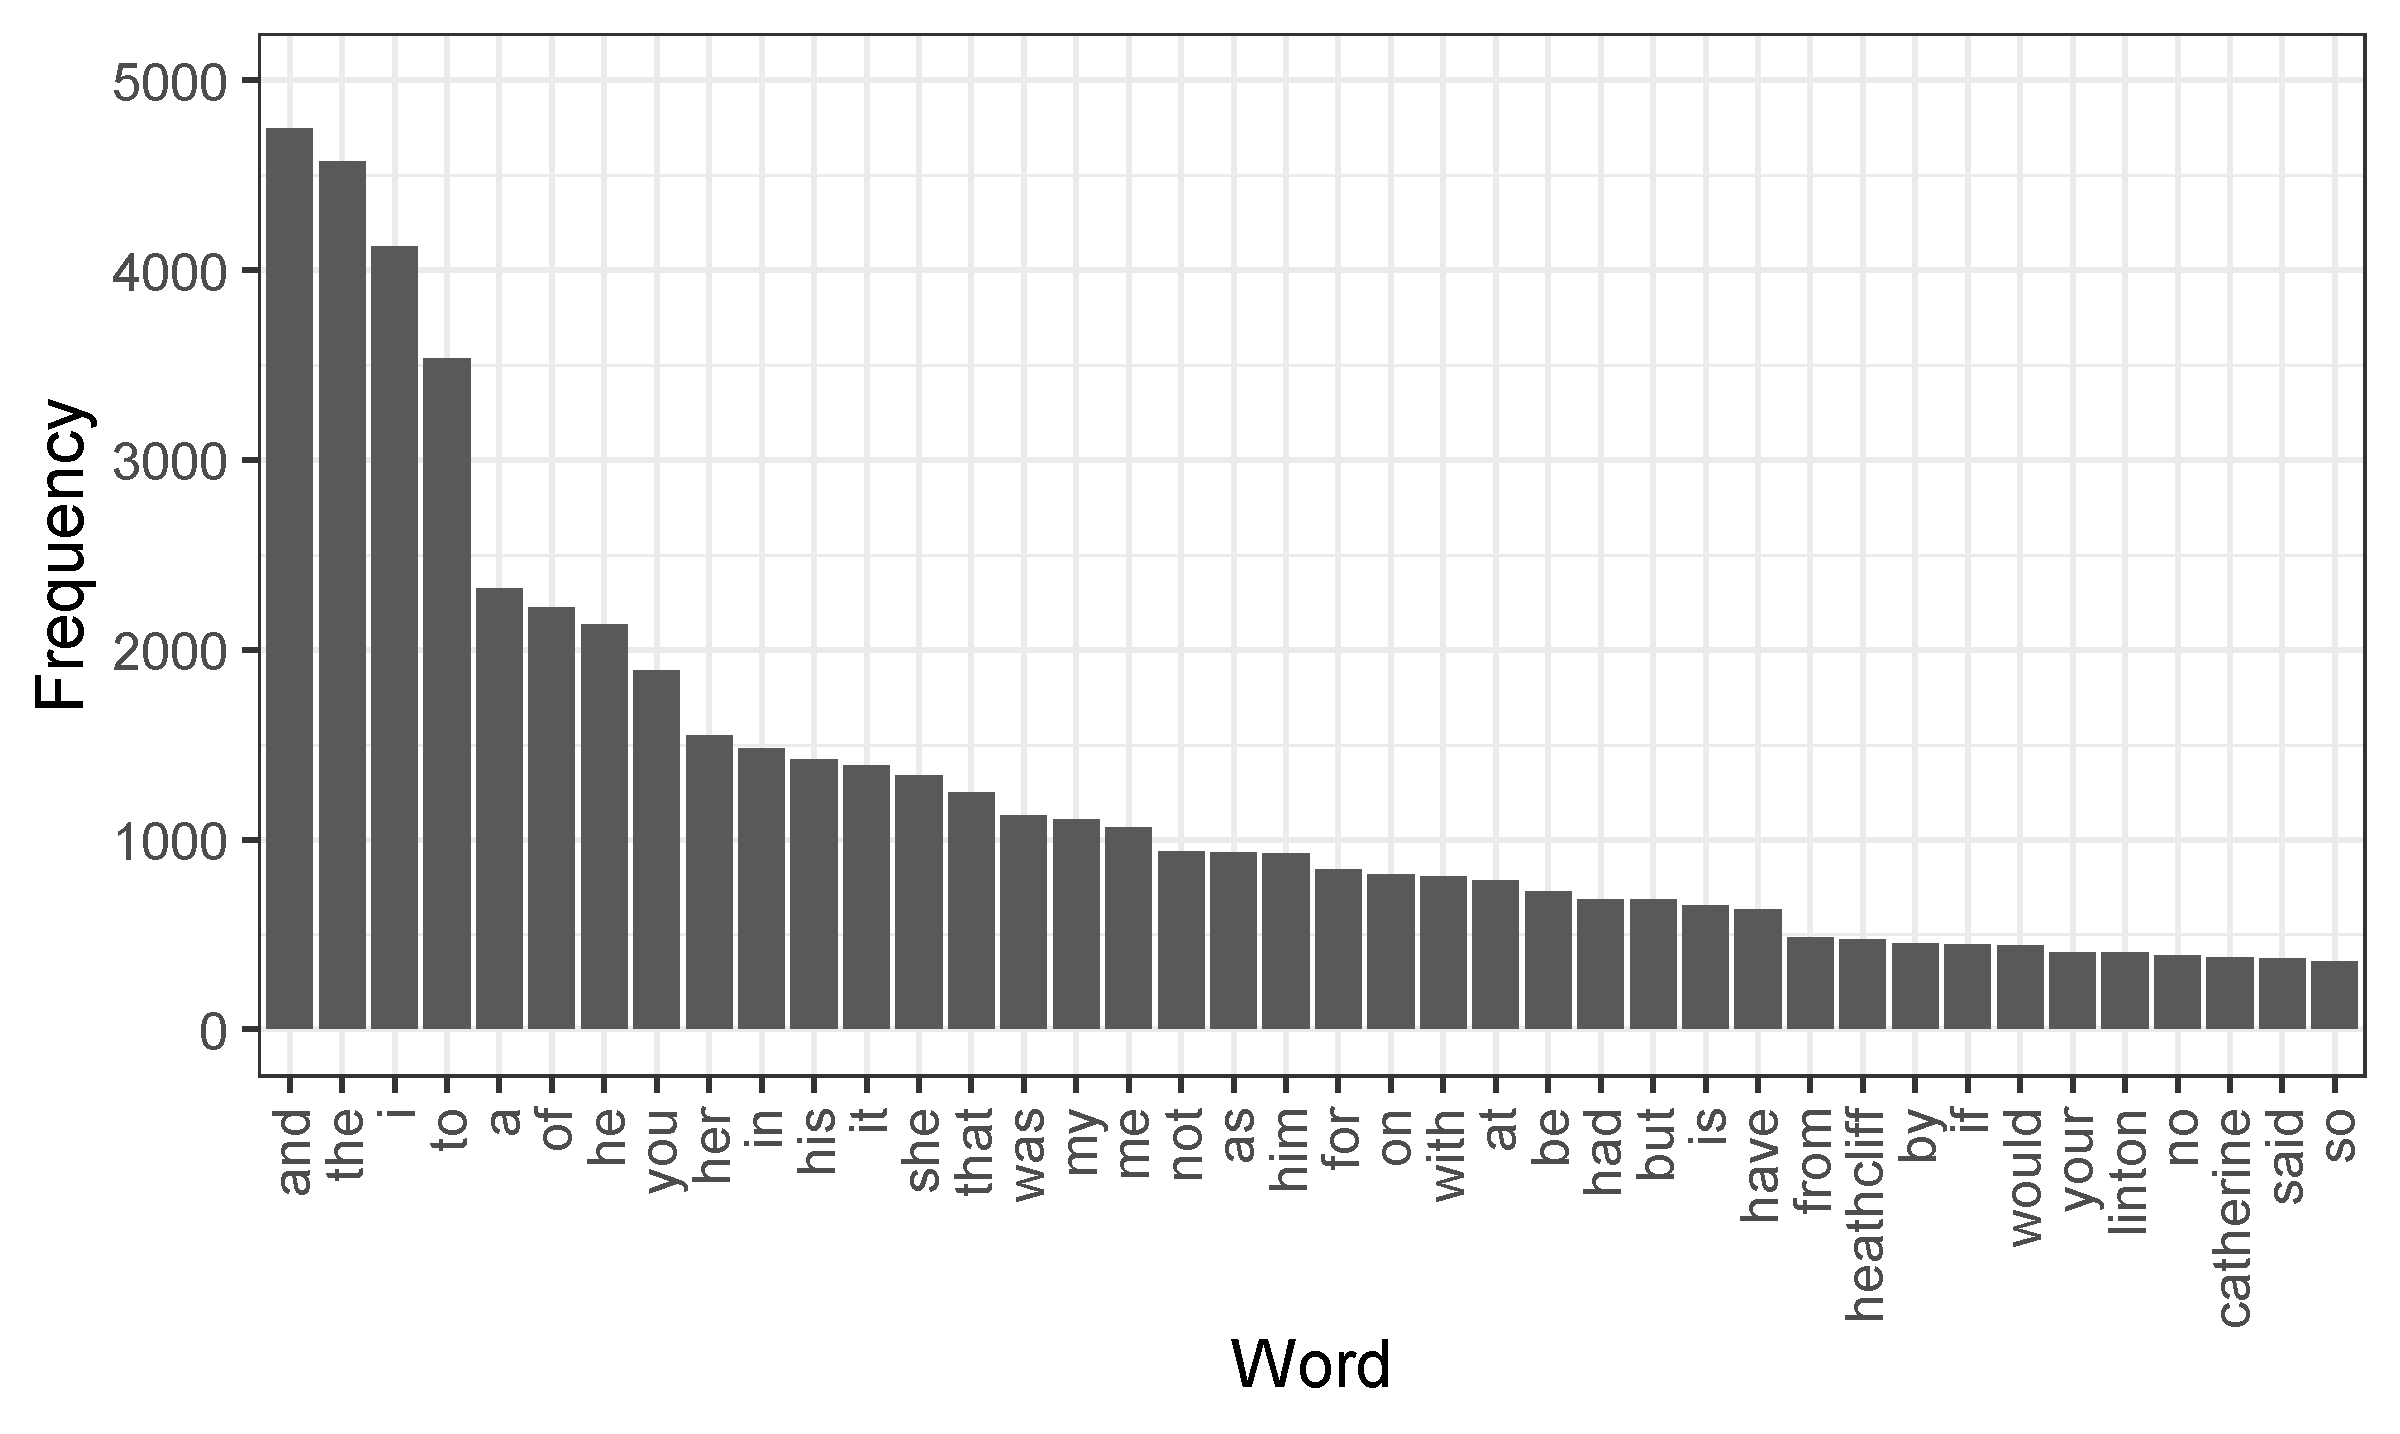
\includegraphics[width=0.90\textwidth]{Figures/corpus_graph.png}
	%\caption{write the title here}
\end{figure}
\end{frame}

% ---------------------------------------------------------------------------

\begin{frame}{Existing Stopword Lists}
\begin{itemize}
\item Python NLTK (127 English words, supports 23 languages)
\item $\mathsf{R}$ package \texttt{stopwords} (175 English words, 231 German words)
\item List of $\sim$ 500 removes 40-50\% of corpus.~\cite{schofield2017pulling}
	\bigskip
\item Project Gutenberg: 60,000+ publicly available e-books\footnote{\url{https://www.gutenberg.org/}}
\item Choose an e-book of general content (e.g. \textit{Alice's Adventures in Wonderland}) to filter out non-technical words from a technical database.~\cite{brooke2015gutentag}
	\bigskip
\item \textbf{Recommendation: Start with a smaller stopword list,\\
	then gradually add more stopwords if necessary.}
\item Words removed do not return to the text model later.
\end{itemize}
\end{frame}

% R code for the package \texttt{stopwords}: 
% stopwords('en'), stopwords('de')

% Python code:
% from nltk.corpus import stopwords
% stopwords.fileids() # file-ids
% ['arabic',  'azerbaijani', 'danish',  'dutch', 'english',
% 'finnish', 'french', 'german', 'greek', 'hungarian',
% 'indonesian', 'italian', 'kazakh', 'nepali', 'norwegian',
% 'portuguese', 'romanian', 'russian', 'slovene', 'spanish',
% 'swedish', 'tajik', 'turkish'] => 23 languages

% ---------------------------------------------------------------------------

\begin{frame}{Removing Stopwords: Known Issues}
\begin{itemize}
\item Beware: Unintentional removal of important information\\
	e.g. ``The The'' (a band), ``to be or not to be'' from \textit{Hamlet}\\
	e.g. ``Chemistry is not easy.'' $\Rightarrow$ ``Chemistry easy.'' (Really?)
\item Most stopword lists contain negation (``no'', ``not'', ``isn't'', etc.).\\
	At a minimum, remove these terms to \textbf{preserve negation}!
	\bigskip
\item Stopwords have syntactic information for \textbf{dependency parsing}.\footnote{~\cite{elming2013down, poria2014dependency}}
\item Patterns of stopword usage help in \textbf{authorship attribution}~\cite{arun2009stopword} and \textbf{plagiarism detection}~\cite{stamatatos2011plagiarism}.
\item Feature: How often pronouns are used for a specific name \footnote{~\cite{sanchez2019paraphrase}}
\item Feature: A person $\Rightarrow$ ``he/she'' or ``he (she)'' or else?
\end{itemize}
\end{frame}

\subsection{Stemming and Lemmatization}

\begin{frame}{Stemming and Lemmatization: Overview}
\begin{itemize}
\item Both stemming and lemmatization normalize words to their base forms for vocabulary consolidation.~\cite{manning2008introduction}
\item A word may have inflectional or derivational morphemes.
	\begin{itemize}
	\item Inflectional: enjoy (verb) $\rightarrow$ enjoy\textbf{s}, enjoy\textbf{ed} (verb)
	\item Derivational: enjoy (verb) $\rightarrow$ enjoy\textbf{able} (adjective)
	\item Derivations change the word's part-of-speech; inflections do not.\footnote{\url{https://blogs.umass.edu/anyman/files/2020/04/Inflectional-vs.-Derivational-Morphemes.pdf}}
	\end{itemize}
	\bigskip
\item Vocabulary consolidation decreases noise in the corpus\\
	e.g. worry, worries, worried, worrying $\rightarrow$ worri
\item Improves performance for \textbf{text classification}~\cite{biba2014boosting} and \textbf{information retrieval}~\cite{rajput2015survey}
\item But risks losing \textbf{semantic information in word variations}\\
	Some sentiments and named entities may be destroyed
	\vspace{-2.5pt}
	\begin{flushright}
	~\cite{bao2014role, cambria2017sentiment}
	\end{flushright}
\end{itemize}
\end{frame}

% R SnowballC: wordStem function
% object, objective, objection -> object
% defend, defender -> defend
% defense -> defens
% respond -> respond
% response, responsible -> respons

% https://nlp.stanford.edu/IR-book/html/htmledition/stemming-and-lemmatization-1.html

\begin{frame}{Stemming and Lemmatization: Comparison}
\begin{itemize}
\item Stemming uses suffix rules to return each word to its root (stem),\\
	and removes both inflectional and derivational variations.
\item Stemming algorithms:~\citet{porter1980algorithm},~\citet{lovins1968development}, Lancaster\footnote{~\cite{paice2005lancaster}}
\item Fast and requires less context, but creates tokens (not real words)\\
	e.g. challenge $\rightarrow$ \textbf{challeng}, president $\rightarrow$ \textbf{presid}
	\bigskip
\item Lemmatization maps a word's inflected forms to its lemma, and considers the part-of-speech.~\cite{bergmanis2018context}
\item Tool: Python NLTK \texttt{WordNetLemmatizer}
\item Isolated word: return the most common lemma or multiple options
\item Helpful in morphologically rich languages (e.g. Turkish, Finnish),\\
	where word changes indicate subject / verb / object / etc.
	\vspace{-2.5pt}
	\begin{flushright}
	~\cite{tsarfaty2010statistical}
	\end{flushright}
\end{itemize}
\end{frame}

\begin{frame}{Stemming and Lemmatization: Potential Risks}
\begin{itemize}
\item\textbf{Over-consolidation}: Words of different meanings $\rightarrow$ same token\\
	``computer'', ``computation'' $\rightarrow$ ``comput'' ($\mathsf{R}$ package \texttt{SnowballC})
\item Some words have multiple lemmas, and context is needed.\\
	``leaves'' $\rightarrow$ ``leave'' (verb, or noun as days off from a job)\\
	``leaves'' $\rightarrow$ ``leaf'' (noun, as on the tree)
	\bigskip
\item\textbf{Sentiment analysis}: Positive \& negative words grouped together\footnote{~\cite{ghazvinian2011star}}\\
	``objective'' (positive), ``objection'' (negative) $\rightarrow$ ``object''
\item\textbf{Named entity recognition}: Entities may become unrecognizable\\
	``Guns N' Roses'' $\rightarrow$ ``gun n rose''~\cite{cambria2017sentiment}
\end{itemize}
\end{frame}

\subsection{N-Gramming and Multi-Word Expressions}

\begin{frame}{N-Gramming: Retain Word Order}
\begin{itemize}
\item N-gramming creates n-grams as phrases of $n$ consecutive words, with a moving window of length $n$ across the text.\footnote{~\cite{gries2010lexical}}
\item Some n-grams are \textbf{multi-word expressions}, and should be retained as a single token. e.g. New Jersey, Black Lives Matter
	\bigskip
\item Word order is important in languages with few inflections.\\
	English: ``dog bites man'' vs ``man bites dog''~\cite{haspelmath1996word}
\item Languages with lots of inflections $\Rightarrow$ word order rarely matters\\
	Latin: Noun as subject has a different form than noun as object.\\
	But word order info is still helpful for context.~\cite{beier2011exploiting}
\end{itemize}
\end{frame}

\begin{frame}{Detecting Multi-Word Expressions: Methods}
\begin{itemize}
\item \textbf{Practical significance}: Threshold of raw frequency\\
Microsoft Azure ML Studio sets 5 times as the default threshold.\footnote{\url{https://tinyurl.com/microsoft-n-grams}}\\
Threshold of 100 times for a corpus of $\sim$1 billion words\footnote{~\cite{berberich2013computing}}
\item \textbf{Statistical significance}: Conditional probability~\cite{chai2017phdthesis}\\
Bi-gram $w_1 w_2$ is a multi-word expression when $P(w_2 | w_1) > P(w_2)$
% Likelihood ratio test?
	\bigskip
\item \textbf{Conditional random fields}{\footnotesize~\cite{lafferty2001conditional, maldonado2017detection}}\\
	Undirected probabilistic graphical model for pattern recognition
% Applications in pattern recognition and machine learning => structured prediction
% https://en.wikipedia.org/wiki/Conditional_random_field
\item \textbf{Retrain word embeddings} to identify multi-word expressions\\
	Still a growing field in deep learning.~\cite{ashok2019comparing}\\
	Tokenizing multi-word expressions does not negatively impact machine translation of single words.~\cite{otani2020pre}
\end{itemize}
\end{frame}

\begin{frame}{Detecting Multi-Word Expressions: Applications}
\begin{itemize}
\item Bag-of-words models: Disregards grammar and word order
\item \textbf{Topic modeling, text classification, information retrieval}
\item Multi-word expressions produce stronger signals.\footnote{~\cite{blei2009visualizing}}
% Bag-of-words models are common! Don't account for word order
% https://en.wikipedia.org/wiki/Bag-of-words_model
	\bigskip
\item Natural language processing tasks where context is required
\item \textbf{Word sense disambiguation}: Determine which meaning of the word is used in a given context~\cite{finlayson2011detecting}
% http://www.scholarpedia.org/article/Word_sense_disambiguation
\item \textbf{Machine translation}: Improves translation accuracy~\cite{tan2014manawi} and extends to multi-lingual corpora~\cite{han2020multimwe}
\item \textbf{Psycholinguistics} (linguistics + psychology):\\ 
	Idiom usage reflects mental representation~\cite{muller2011multi}
\end{itemize}
\end{frame}

\section{Dataset Examples}

%\frame{\tableofcontents[currentsection]}
\frame{\tableofcontents[currentsection, hidesubsections]}

\subsection{Example 1: JSM Abstract Dataset}

% JSM = Joint Statistical Meetings
% Topic modeling + keywords
% -> Conference session scheduling

% 1st slide: Text preprocessing
% 2nd slide: Applications

\begin{frame}[fragile]{Example 1: JSM Abstract Dataset -- Preprocessing}
  \hspace{-45pt}
  \vspace{-30pt}
\begin{itemize}
\item Dataset: 3000+ abstracts and 700+ sessions from JSM 2015\\
	\textbf{JSM (Joint Statistical Meetings)} is a large global conference.
\item Lots of technical terms: e.g. maximum likelihood estimation
\item \textbf{Extract technical terms for conference session scheduling}
\end{itemize}
	\vspace{10pt}
\begincols
  %\hspace{-30pt}
  \begincol{.55\textwidth}
Stopword removal process:~\cite{yongjianbi2016masters}
\begin{enumerate}
\item Stem and n-gram\\ the JSM dataset.
\item Stem and n-gram an e-book\\ from Project Gutenberg.
\item Remove anything from 1.\\ that exists in 2.
\end{enumerate}
  \endcol
  \hspace{-75pt}
  \begincol{.55\textwidth}
  \vspace{-15pt}
% Add a Venn diagram in LaTeX for JSM dataset x Project Gutenberg (done)

% Example code: 
% https://www.reddit.com/r/LaTeX/comments/i4xv1k/help_with_venn_diagramms/
% https://www.latex4technics.com/?note=XTM

\def\firstcircle{(0,0) circle (2.5cm)}
\def\secondcircle{(0:2.5cm) circle (2.5cm)}
\colorlet{circle edge}{black!75}
\colorlet{circle area}{gray!33}
\tikzset{filled/.style={fill=circle area, draw=circle edge, thick},
    outline/.style={draw=circle edge, thick}}

\begin{figure}[!ht]
\centering
\begin{tikzpicture}[transform canvas={scale=0.75}]
    \begin{scope}
        \clip \firstcircle;
        \fill[filled] \secondcircle;
    \end{scope}
    \draw[outline] \firstcircle;
    \node[align=center] (A) at (-1cm,0) {JSM \\ abstract \\ collection};
    \draw[outline] \secondcircle ;
    \node[align=center] (B) at (3.5cm,0) {Project \\ Gutenberg};
    \node[below,text width=1cm,align=center,anchor=center] at (barycentric cs:A=1/2,B=1/2){Removed \\ from \\ corpus};
\end{tikzpicture}
%\caption{Intersection with Project Gutenberg is removed from the JSM abstract collection.}
%\label{fig:venn-diagram}
\end{figure}
  \endcol
\endcols
\hspace{100pt}
\end{frame}

\begin{frame}{Example 1: JSM Abstract Dataset -- Applications}
% LDA (latent Dirichlet allocation) identified six topics
% List the six topics here

% Conference session scheduling
% Minimize the overlap of sessions with similar topics
% So that people interested in a topic can attend most of the relevant sessions
% Automated system is still needed (cite more recent talks)
% Virtual conferences: People can still watch recordings
% => cite the numbers of recordings being watched
\begin{itemize}
\item Topic models: Six topics found by LDA (latent Dirichlet allocation)\\
	Spatial stats, clinical trials, Bayesian, genomics, hypothesis tests
	\bigskip
\item Conference session scheduling:\\
	\textbf{Minimize the overlap of sessions with similar topics}\\
	\textbf{People interested in a topic can join many relevant sessions}
\item Abstracts often include keywords from authors, but an automated system is still needed for session scheduling.~\cite{sweeney2020unsupervised}
	\bigskip
\item \textbf{Virtual conferences: Scheduling is still a challenge!} \footnote{~\cite{patro2020fair}}\\ 
	Without physical restrictions, but need to account for other factors.\\
	% e.g. time zones, sign language interpreter availability, etc.
	Availability of on-demand recordings may change the equation.
\end{itemize}
\end{frame}

\subsection{Example 2: Social Media Data}

% Unsure if I still need the Twitter data subsection,
% because I really don't have actual data as example.
% => Decided to keep this example!
% Still want to show some trends e.g. social movements~\cite{marshall2018impact}

% NLTK tokenizer
% TweetTokenizer(): retains Twitter hashtags and emoticons
% (give an example here)
% https://www.nltk.org/api/nltk.tokenize.html

% Do I need to talk about data collection?
% Python tweepy and R twitteR // especially for Twitter
% https://utstat.toronto.edu/~nathan/teaching/sta4002/Class1/scrapingtwitterinR-NT.html

% R package rvest, the Python library scrapy, or the Google Web Scraper.
% https://webscraper.io/
% Google Web Scraper Tutorial
% https://medium.com/@luxii/google-web-scraper-tutorial-4efa89608d89


\begin{frame}{Example 2: Social Media Data -- Preprocessing}
\begin{itemize}
% Data Collection
\item Twitter: Twitter developer API, Python \texttt{tweepy}, $\mathsf{R}$ \texttt{twitteR}
\item Webscraping: Python \texttt{scrapy}, $\mathsf{R}$ \texttt{rvest}, webscraper.io, etc.
	\bigskip
\item Remove HTML tags: Python \texttt{BeautifulSoup}, $\mathsf{R}$ \texttt{textclean}
\item Remove leading and trailing whitespaces for each message
\item Python NLTK \texttt{TweetTokenizer()}\footnote{\url{https://www.nltk.org/api/nltk.tokenize.html}} retains hashtags (\texttt{\#hashtag}), mentions (\texttt{@username}), and emoticons (\texttt{:-D})
	\bigskip
\item Text normalization: Consider splitting Internet slang abbreviations\\
	e.g. cu = see you, idk = I don't know~\cite{pennell2011toward} 
\item Dependency parsing: Beware of nonstandard spellings and punctuation usage~\cite{blodgett2018twitter}
\end{itemize}
\end{frame}

% Lots of applications... but these cannot be done without data preprocessing.
% (I don't think data preprocessing is the first step, because we need to define the problem statement beforehand.)

% How social media data is used for COVID responses
% emergency response, major incidents
% Business applications (not very important during the pandemic)
\begin{frame}{Example 2: Social Media Data -- Applications}
\begin{itemize}
\item \textbf{COVID-19}: Information spreading~\cite{cinelli2020covid}\\
Twitter dataset with daily updates~\cite{banda2020large}\footnote{\url{https://github.com/thepanacealab/covid19_twitter}}\\
COVID-Twitter-BERT: Pretrained large corpus{\small~\cite{muller2020covid}\footnote{\url{https://github.com/digitalepidemiologylab/covid-twitter-bert}}}
	\bigskip
\item \textbf{Analyze the Event Impact}:\\
	Black Lives Matter~\cite{giorgi2020twitter}\\
	2020 US presidential election~\cite{chen2020election2020}\\
	National Disaster Situational Awareness~\cite{karami2020twitter}
	\bigskip
\item But applications cannot be done without \textbf{text preprocessing}.\\
	Data need to be preprocessed to be ready for text model input.
\end{itemize}
\end{frame}

\subsection{Example 3: Text with Numerical Ratings}

\begin{frame}{Example 3: Text with Numerical Ratings -- Data}
\begin{itemize}
\item Employee satisfaction survey:~\cite{Chai2019Text}\\
	Ratings from \textbf{1 (least satisfied)} to \textbf{10 (most satisfied)}\\
	Text comment to explain why you made the rating
\item Best: Combined analysis in text and numerical data
	\bigskip
\item Need to \textbf{preserve negation terms} while removing stopwords.\\
	``No clear path to promotion'' $\Rightarrow$ ``Clear path promotion''?\\
	Negation terms should be excluded from the stopword list.
	\bigskip
\item Data often contain possible errors.\\ 
	``Love my work -- very varied.'' $\Rightarrow$ rating 1?\\
	Common reason: \textbf{Confusion with rating scale}~\cite{fisher2013analytics}\\
	The respondent meant 10 (most satisfied) but reverted the scale.
\end{itemize}
\end{frame}

\begin{frame}{Example 3: Text with Numerical Ratings -- Modeling}
\begin{itemize}
\item How to \textbf{detect potential rating errors} in the survey?
	\bigskip
\item \textbf{Method 1: Leverage the text response} (i.e., text mining)\\
	Predict the rating from the text comment with supervised methods\\
	Large discrepancy between predicted rating and actual rating\\
	$\Rightarrow$ Flag as potential error and examine the record
	\bigskip
\item \textbf{Method 2: Leverage other ratings} in the same dataset\\
	Predict the overall rating from the ratings of each item\\
	e.g. EM (expectation maximization) algorithm{\footnotesize~\cite{fisher2011getting}}\\
	Also check for large discrepancies between predicted and actual 
\end{itemize}
\end{frame}
% Text mining => detect potential rating errors
% sLDA [citation needed]
% EM algorithm (expectation maximization) [citation needed]
% when there are other ratings in the same survey
% Replace the rating $C$ with $11-C$


\subsection{Example 4: Biomedical Data}

% State that clinical text is a sublanguage~\cite{temnikova2013closure}
% Word embeddings do not always contain biomedical terms [citation needed]

% Clinical text in Bulgarian: ``/'' (forward slash) is an important characteristic~\cite{temnikova2013closure}

% ``Violations of univocality: two semantically similar terms with different structure in their term labels.''
% https://themindwobbles.wordpress.com/2009/06/29/pto6-ontology-quality-assurance/

% Some word embeddings for biomedical NLP, but not much yet

% Train word embeddings on biomedical publications (e.g. PubMed)~\cite{wang2018comparison}
% BioBERT~\cite{lee2020biobert}

% Biomedical word embeddings with GloVe
% ``distinct vector to represent each word and ignores the internal structure of words''
% ``deltaproteobacteria'' vs ``betaproteobacteria''~\cite{zhang2019biowordvec}
% https://www.nature.com/articles/s41597-019-0055-0

\begin{frame}{Example 4: Biomedical Data}
\begin{itemize}
\item Pretrained word embeddings for biomedical text\\ 
	Gradually increasing in popularity~\cite{wang2018comparison}\\
	BioBERT~\cite{lee2020biobert}: Pretrained on PubMed and PMC
\item Challenge: Word vectors don't reflect internal structure of words.\\
	e.g. ``\textbf{delta}proteobacteria'' and ``\textbf{beta}proteobacteria'' are related.\\
	$\Rightarrow$ Leverage subword info. in pretraining~\cite{zhang2019biowordvec}
	\bigskip
\item Tokenizing biomedical text includes \textbf{Greek letter normalization} and \textbf{break point identification}~\cite{jiang2007empirical}
\item Both \texttt{MIP-{\color{red}\textbf{1-}\boldmath{$\alpha$}}} and \texttt{MIP-{\color{red}\textbf{1}\boldmath{$\alpha$}}} should tokenize to \texttt{MIP 1 alpha}
% \item Both \texttt{MIP-{\color{red}1-$\alpha$}} and \texttt{MIP-{\color{red}1$\alpha$}} should tokenize to \texttt{MIP 1 alpha}
\item Text string \texttt{NF-$\kappa$ B/CD28-responsive}{\small~\cite{trieschnigg2007influence}}
	\begin{itemize}
	\small
	\item \texttt{nf $\kappa$ b cd responsive}: 32\% precision in document retrieval
	\item \texttt{nf kappa nfkappa b cd 28 respons bcd28respons}: 40\%
	\end{itemize}
\end{itemize}
\end{frame}


\begin{frame}{Example 4: Biomedical Data}
\begin{itemize}
\item NLTK tokenizer + post-processing $\Rightarrow$ fewer tokenization errors
% post-processing = custom script
\end{itemize}
\begin{figure}[!ht]
	\centering
	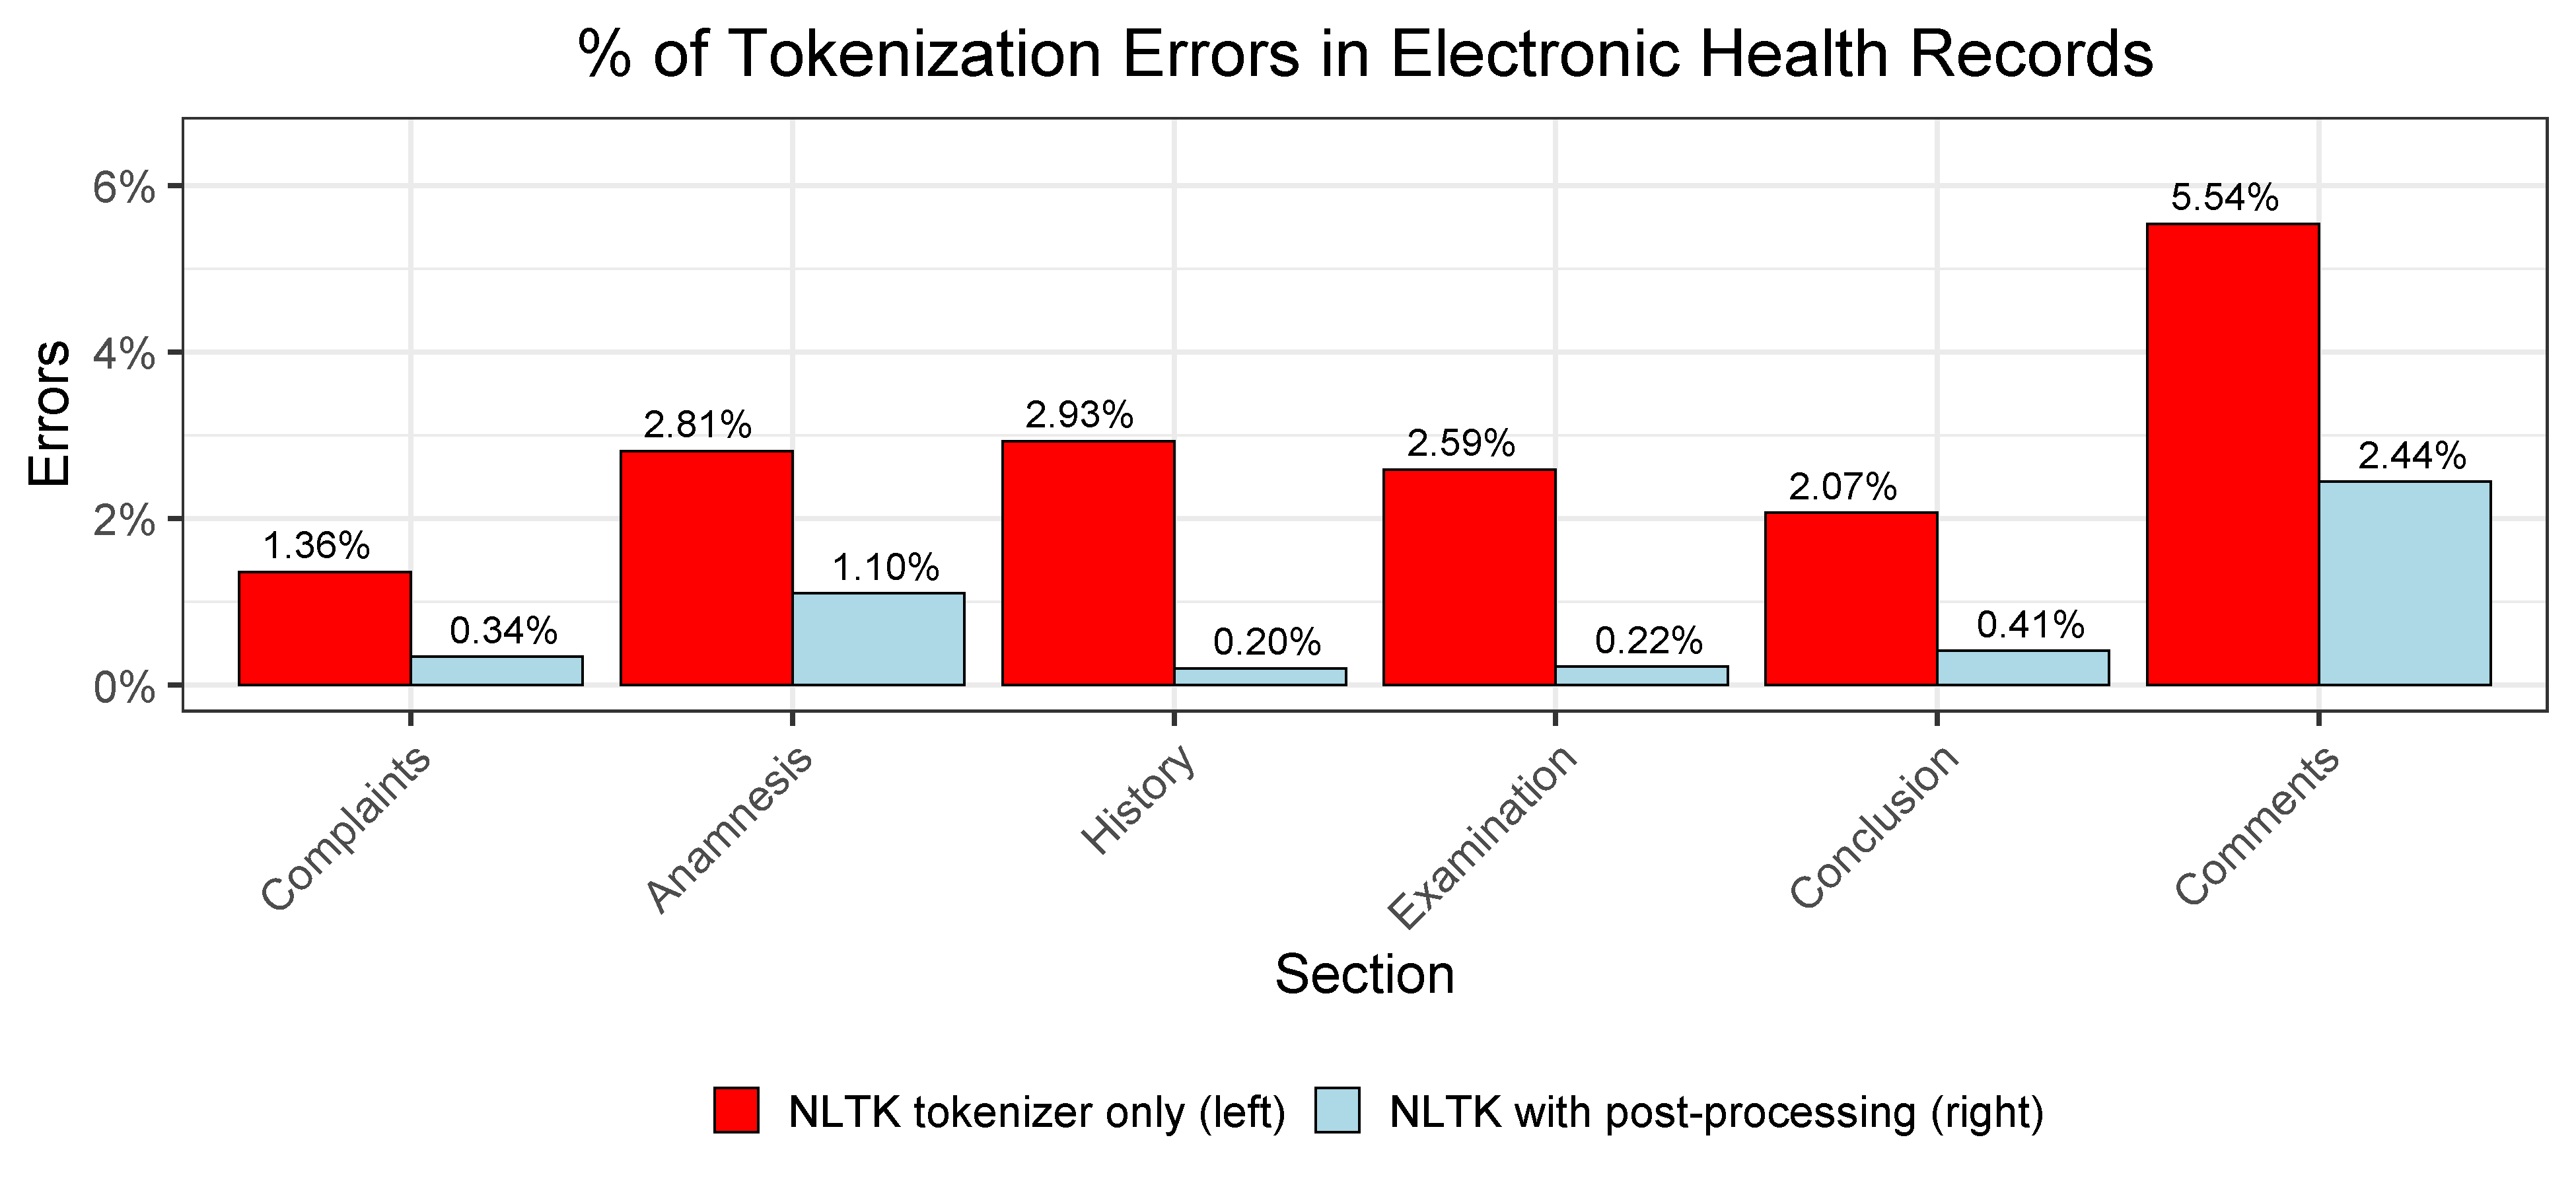
\includegraphics[width=\textwidth]{Figures/gron2018_table1.png}
	%\caption{write the title here}
\end{figure}
\begin{flushright}
Data from Table 1 in~\cite{gron2018clinical}
\end{flushright}
\end{frame}


\section{Discussion and Key Takeaways}

%\frame{\tableofcontents[currentsection]}
%\frame{\tableofcontents[currentsection, hidesubsections]}

\begin{frame}{Discussion}
\begin{itemize}
\item Different applications require different preprocessing methods.
	\bigskip
\item Bag-of-words models: Acceptable to remove punctuation, remove stopwords, stem and lemmatize the corpus.
	\begin{itemize}
	\item \textbf{Topic modeling, text classification, information retrieval}, etc.
	\end{itemize}
	\bigskip
\item Other applications that require more context: Need to reconsider whether each text preprocessing step is appropriate.
	\begin{itemize}
	\item \textbf{Dependency parsing, machine translation,\\
		text summarization, question answering}, etc.
	\end{itemize}
	\bigskip
\item Detecting multi-word expressions is a challenging problem,\\
	even with the help of word embeddings.~\cite{park2019learning}
\end{itemize}
\end{frame}

% Bag-of-words models => Acceptable to remove punctuation, remove stopwords, stem and lemmatize the corpus
%	List the three applications: Topic modeling, text classification, information retrieval

% But for other applications,
% e.g. dependency parsing, machine translation, text summarization, question answering, etc.
% The more context needed => keep more semantic information in the corpus
% Need to reconsider whether each text preprocessing step is appropriate

% Detecting multi-word expressions is still a challenging research problem.

% NLP is not just English, lots of other languages exist! 
% with different linguistic characteristics
% May require different preprocessing methods

\begin{frame}{Key Takeaways}
\begin{itemize}
\item Text preprocessing prepares the corpus for analysis,\\
	so this directly affects data quality in modeling.
\item Document the decisions made in the process~\cite{nugent2020instead}
	\bigskip
% If you remember just one thing from the talk, this would be ...
\item \textbf{Exclude negation terms from the stopword list!}\\
	Don't accidentally remove negation from the corpus.
% (minimum recommendation)
	\bigskip
\item Word embeddings are useful, but not a panacea solution.\\
	A non-trivial prerequisite: Tokenize the corpus into words\\
	% e.g. tokenize corpus into words, minority languages, biomedical text
\item Need to learn text preprocessing basics to make better decisions.
\end{itemize}
\end{frame}

\begin{frame}{Acknowledgments}
\begin{itemize}
\item I am grateful for the support of \textbf{Microsoft}.
\item (Insert colleague names here)
	\bigskip
\item I'd like to thank \textbf{Prof. David Banks}, my PhD advisor at Duke University, who motivated me to do research in text preprocessing.
\item I also thank my friend \textbf{Sourav Sen} for feedback on the slides.
	\bigskip
\item I declare that there is no conflict of interest.
\end{itemize}
\end{frame}

\hypersetup{bookmarksdepth=-1} % Exclude bookmarks from this section
\section{References}
\hypersetup{bookmarksdepth} % back to default

\begin{frame}[t,allowframebreaks]{References}
\footnotesize
\bibliographystyle{apalike}
\bibliography{References_CSP2021_ChristineChai}
\end{frame}

% LAST PAGE
%\begin{frame}{Q\&A}
%\huge Thank you for your attention!
%\end{frame}

\end{document}